\chapter{Introduction}
\label{sec:introduction}

\section{Problem statement}
\label{sec:prob_stmt}

\begin{figure}
  \centering
  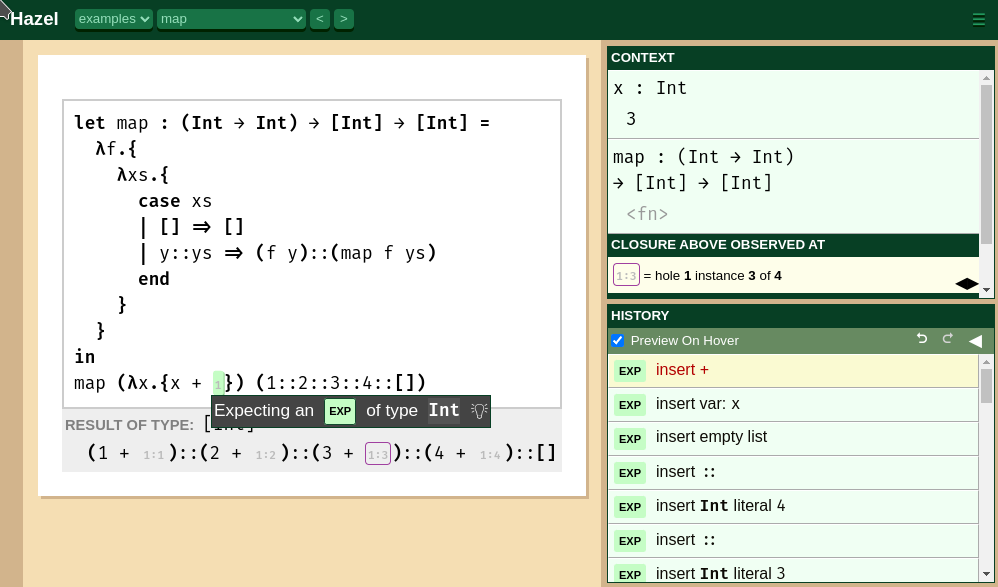
\includegraphics[width=4in]{img/hazel_ui.png}
  \caption[Screenshot of the Hazel live programming environment.]{A screenshot of the Hazel live programming environment. Screenshot taken of the dev branch demo on 02/06/2022 \cite{HazelDemo2022}.}
  \label{fig:screenshot-hazel-ui}
\end{figure}

Unstructured plaintext editing has remained the dominant mode of programming for decades, but makes it more difficult to implement editor services to aid the process. Structural editors, on the other hand, only allow valid edit states. Several structural editors \todoref{structural editors} have been proposed to improve the programming experience and introduce editor services, such as the elimination of syntax errors or graphical editing.

Hazel \cite{Hazel2022} is an experimental structural language definition and implementation that aims to solve the ``gap problem'': spatial and temporal holes that temporarily prevent code from being able to be compiled or evaluated. The structural editor is defined by a bidirectional edit calculus Hazelnut \cite{conf/popl/Hazelnut17}, which governs the structural editor and the static semantics (typing rules) of the language. The dynamic semantics (evaluation semantics) are described in \cite{conf/popl/HazelnutLive19}.

Hazel is a relatively new research effort by the University of Michigan's Future of Programming Lab (FPLab), with little effort placed on performance optimizations. This work attempts to achieve several enhancements that will benefit the performance of evaluation and related tasks. Part of the work will be the standard conversion from evaluation using the substitution model (simpler to reason about) to the environment model (more performant) \todoref{standard conversion}, with emphasis on evaluation of holes and postprocessing of the evaluation result to match the result from evaluation with substitution. The latter parts of this work will use the environment model of evaluation to improve the memoization of certain tasks related to Hazel's structure (such as hole closure numbering), and also implement the fill-and-resume performance enhancement described in \cite{conf/popl/HazelnutLive19}. The novelty of this work lies in the novelty and optimization opportunity of Hazel's hole-based static and dynamic semantics.

\section{The contribution of this work}
\label{sec:contribution}

This thesis presents several algorithms designed for Hazel's evaluation:
\begin{itemize}
\item The evaluation semantics of the Hazel language using the environment model (which replaces the substitution model as implemented on the trunk branch and described in \cite{conf/popl/HazelnutLive19}). While most of this is standard, we aim to keep the implementation pure (which is less trivial in the case of recursion), introduce uniquely-numbered environments (for later use in memoization), and describe the evaluation of holes (which are unique to Hazel).
\item Postprocessing, which is memoized by environments and has the dual functions of converting the result to the equivalent result from evaluation with substitution, and performing hole closure numbering. Converting the result to the substitution model, hole closure numbering, and memoization of environments are all described separately.
\item Fill-and-resume, as originally proposed in \cite{conf/popl/HazelnutLive19}. This algorithm is described at a high level in the original description and not yet implemented until this thesis work. We provide the implementation and a lower-level description of said implementation.
\end{itemize}
The first two algorithms will be provided as a series of (big-step) inference rules, in the same style as the existing literature. Fill-and-resume will be presented at a higher level, being more of a composition of existing functions of the Hazel architecture.

In addition to the algorithms above, several core concepts or data structures are introduced to Hazel, such as unique hole closures (as opposed to hole instances) and generalized closures. While the first one is specific to holes and thus specific to Hazel(nut), the latter is a concept that may be transferred to any live environment that may perform a similar conversion between evaluation with environments (for evaluation performance) to a result using substitution (for display and debugging purposes).

The performance of this work is measured primarily in terms of empirical performance gains (via evaluation-step counting and benchmarking), and discussed with respect to the theoretical performance. This proof of correctness of the algorithms was not mechanized in the Agda proof assistant as was much of the core of Hazelnut \cite{conf/popl/Hazelnut17} and Hazelnut Live \cite{conf/popl/HazelnutLive19}. Instead, correctness of implementation is validated by standard software testing procedures with manual test cases, and a mechanized proof is deferred for future work.

\section{Structural overview}
\label{sec:structural_overview}

\Cref{sec:prog_lang_principles} provides a background on necessary topics in programming language (PL) theory and programming language implementations, in order to frame understanding for the Hazel live programming environment. \Cref{sec:hazel} provides an overview of Hazel, in order to frame the work completed for this thesis project. \Crefrange{sec:env_model_evaluation}{sec:far_impl} describe the primary work completed for this project, as described in \Cref{sec:contribution}. \Cref{sec:evaluation} comprises an assessment of the work completed in terms of correctness and the theoretical performance. \Cref{sec:future_work} is a discussion of future research directions that may be spawned off from this work. \Cref{sec:concl} concludes with a summary of findings and future work. The Appendices contain additional information about the Hazel project not directly related to the primary contribution of this project, as well as selected source code snippets.

%%% Local Variables:
%%% mode: latex
%%% TeX-master: "main"
%%% End:
